\documentclass[11pt,a4paper]{ctexart}

\usepackage[a4paper,margin=2.35cm]{geometry}
\usepackage{amsmath,amssymb,amsthm,mathtools}
\usepackage{booktabs}
\usepackage{array}
\usepackage{xcolor}
\usepackage{hyperref}
\usepackage{tikz}
\usetikzlibrary{arrows.meta,positioning,calc,decorations.pathreplacing}

\hypersetup{
  colorlinks=true,
  linkcolor=blue!60!black,
  urlcolor=blue!60!black,
  citecolor=blue!60!black
}

\setCJKmainfont{Noto Serif CJK SC}
\setCJKsansfont{Noto Sans CJK SC}
\setmonofont{DejaVu Sans Mono}

\newcommand{\Fp}{\mathbb{F}_p}
\newcommand{\ZZ}{\mathbb{Z}}
\newcommand{\supp}{\operatorname{Supp}}
\newcommand{\ord}{\operatorname{ord}}

\theoremstyle{definition}
\newtheorem{definition}{定义}
\newtheorem{claim}{命题}
\newtheorem{theorem}{定理}
\newtheorem{remark}{说明}

\title{\bfseries Order-Four Sparse Cleaner：\\
BGV 二代自举中多项式优化的数学来源}
\author{实验说明稿}
\date{\today}

\begin{document}
\maketitle

\begin{abstract}
这份说明解释本实验中最核心的优化技巧：在大素数 BGV 自举的
bounded-support digit-cleaning 问题里，不再试图对同一个固定 support
寻找更低次数的 exact polynomial，而是选择一个具有四阶对称性的辅助 radix
$A$。当 $p=65537$ 且 $A=256$ 时，有
\[
  A^2 \equiv -1 \pmod p.
\]
因此乘以 $A$ 在 support 坐标 $(h,\ell)$ 上等价于一次 $90^\circ$ 旋转。
这个旋转对称性强迫 exact cleaner 的单项式指数只可能落在
$X$ 和 $X^{4j+3}$ 上，于是
\[
  P_A(X)=c_1X+X^3Q(X^4).
\]
这既解释了 cleaner 从 $612$ 项降到 $307$ 项的代数原因，也解释了为什么
可以设计一个专用 evaluator。以 \texttt{/baselines/BGV-Boot-for-Large-p}
为正式对比对象，真实 HElib 自举中的 digit extraction 从 $160.78$s
降到 $80.77$s。
\end{abstract}

\tableofcontents

\section{问题背景：自举里的 exact cleaner}

在大素数 BGV bootstrapping 中，线性变换之后的 slot 中可以看成含有一个
小噪声范围内的整数。为了把密文刷新，需要同态地做一次类似
``取低位'' 或 ``清除高位'' 的操作。本文实验关心的是如下有限域上的
restricted exact cleaning 问题。

\begin{definition}[辅助 radix 与 bounded support]
令 $p$ 为明文素数，$A\in \Fp^\ast$ 为辅助 radix，$B$ 为噪声/支撑界。
定义
\[
  S_A=\{hA+\ell \in \Fp:\; h,\ell\in[-B,B]\cap\ZZ\}.
\]
这里 $h$ 是高位坐标，$\ell$ 是低位坐标。
\end{definition}

我们的 cleaner 是一个多项式函数
\[
  C_A:S_A\to \Fp,\qquad C_A(hA+\ell)=\ell.
\]
也就是说，输入是 $hA+\ell$，输出只保留低坐标 $\ell$。

\subsection{一般参数定理：$p$ 能任取到什么程度}

这里要把两个层次分开。第一层是 ``exact cleaner 是否存在并且正确''；
第二层是 ``是否存在本文使用的四阶稀疏结构''。前者对 $p$ 的要求很宽，
后者要求 $p$ 中存在 $\sqrt{-1}$。

\begin{theorem}[任意足够大素数上的 exact cleaner]
\label{thm:generic-prime-cleaner}
令 $B\ge1$，$p$ 为素数，并且
\[
  p>4B(B+1).
\]
取整数代表
\[
  A=2B+1.
\]
则映射
\[
  \phi_A:[-B,B]^2\cap\ZZ^2\longrightarrow \Fp,\qquad
  (h,\ell)\longmapsto hA+\ell
\]
是单射。因此 $|S_A|=(2B+1)^2$，并且存在唯一的次数
$<|S_A|$ 的多项式 $P_A\in\Fp[X]$ 满足
\[
  P_A(hA+\ell)=\ell,\qquad |h|,|\ell|\le B.
\]
\end{theorem}

\begin{proof}
若两个坐标给出同一个域元素，则存在
\[
  u=h-h',\qquad v=\ell-\ell',
\]
其中 $|u|,|v|\le2B$，且
\[
  uA+v\equiv0\pmod p.
\]
若 $u=0$，则 $v\equiv0\pmod p$。由于 $|v|\le2B<p$，只能有 $v=0$。

若 $u\ne0$，由 $A=2B+1$ 得
\[
  |uA+v|\ge A-|v|\ge (2B+1)-2B=1,
\]
同时
\[
  |uA+v|\le 2BA+2B=2B(2B+1)+2B=4B(B+1)<p.
\]
所以 $uA+v$ 是一个非零整数，绝对值严格小于 $p$，不可能被 $p$ 整除。
这与 $uA+v\equiv0\pmod p$ 矛盾。因此只能有 $u=v=0$，映射单射。

单射给出 $|S_A|=(2B+1)^2$。在有限域上，对 $S_A$ 上的任意函数都可以
做 Lagrange 插值，并且存在唯一的次数 $<|S_A|$ 的代表元。因此 exact
cleaner $P_A$ 存在且唯一。
\end{proof}

\begin{theorem}[四阶稀疏 cleaner 的一般定理]
\label{thm:order-four-general}
令 $B\ge1$，$p$ 为奇素数。若
\[
  p\equiv1\pmod4,\qquad p>8B^2,
\]
则 $\Fp$ 中存在元素 $A$ 满足
\[
  A^2\equiv-1\pmod p.
\]
任取这样的 $A$，映射 $\phi_A(h,\ell)=hA+\ell$ 在
$[-B,B]^2$ 上单射。设 $P_A$ 为唯一的次数 $<|S_A|$ 的 exact cleaner，
则存在 $Q\in\Fp[X]$ 使得
\[
  \boxed{P_A(X)=\frac12X+X^3Q(X^4).}
\]
等价地，$P_A$ 的非零单项式只能出现在 $X$ 和指数
$k\equiv3\pmod4$ 的项上。
\end{theorem}

\begin{proof}
先证明 $A$ 的存在性。$\Fp^\ast$ 是阶为 $p-1$ 的循环群。
$A^2=-1$ 的解存在当且仅当 $\Fp^\ast$ 中存在四阶元素，也就是
$4\mid p-1$，等价于 $p\equiv1\pmod4$。

接着证明 support 单射。若
\[
  uA+v\equiv0\pmod p,\qquad |u|,|v|\le2B,
\]
且 $(u,v)\ne(0,0)$，则 $u=0$ 时立即得到 $v=0$，矛盾。所以可设
$u\ne0$。由 $uA\equiv-v$ 得
\[
  u^2A^2\equiv v^2\pmod p.
\]
代入 $A^2=-1$，得到
\[
  u^2+v^2\equiv0\pmod p.
\]
但非零整数 $u^2+v^2$ 满足
\[
  0<u^2+v^2\le (2B)^2+(2B)^2=8B^2<p,
\]
不可能被 $p$ 整除。因此只能有 $u=v=0$，单射成立。

现在取 support 点 $x=hA+\ell$。因为 $A^2=-1$，
\[
  Ax=hA^2+\ell A=\ell A-h.
\]
也就是说，乘以 $A$ 把坐标 $(h,\ell)$ 变为 $(\ell,-h)$，仍然落在
$[-B,B]^2$ 内。于是
\[
  P_A(x)=\ell,\qquad P_A(Ax)=-h.
\]
因此在整个 support 上有
\[
  P_A(Ax)+AP_A(x)=-h+A\ell=Ax.
\]
令
\[
  R(X)=P_A(AX)+AP_A(X)-AX.
\]
由于 $\deg R<|S_A|$，且 $R$ 在 $|S_A|$ 个不同 support 点上为零，
所以 $R$ 是零多项式。

写 $P_A(X)=\sum_k c_kX^k$。比较
\[
  P_A(AX)+AP_A(X)=\sum_k c_k(A^k+A)X^k=AX
\]
的系数。$k=1$ 时有 $2Ac_1=A$，所以 $c_1=1/2$。当 $k\ne1$ 时，
若 $c_k\ne0$，则
\[
  A^k+A=0
  \quad\Longleftrightarrow\quad
  A^{k-1}=-1=A^2.
\]
由于 $A$ 的阶为 $4$，这等价于 $k\equiv3\pmod4$。于是
$P_A(X)=\frac12X+X^3Q(X^4)$。
\end{proof}

\begin{remark}[$p$ 是否可以任取]
如果目标只是 exact cleaner 的正确性，定理~\ref{thm:generic-prime-cleaner}
说明任意满足 $p>4B(B+1)$ 的素数都可以使用，取 $A=2B+1$ 即可。
如果目标是本文的四阶稀疏优化，$p$ 不能完全任取；素数情形必须满足
$p\equiv1\pmod4$，并且为了自动保证 support 无碰撞，一个干净的充分条件是
$p>8B^2$。更小的 $p$ 或其他 $A$ 不是一定不可用，但需要逐点做 collision
check 和 exactness verification。
\end{remark}

\begin{center}
\begin{tikzpicture}[
  box/.style={draw, rounded corners=2pt, align=center, minimum width=34mm, minimum height=10mm},
  arr/.style={-{Latex[length=2mm]}, thick}
]
\node[box, fill=blue!8] (slot) {自举中间值\\$x=hA+\ell$};
\node[box, fill=green!10, right=18mm of slot] (poly) {exact cleaner\\$P_A(x)=\ell$};
\node[box, fill=orange!12, right=18mm of poly] (out) {清理后的低位\\$\ell$};
\draw[arr] (slot) -- (poly);
\draw[arr] (poly) -- (out);
\end{tikzpicture}
\end{center}

\section{固定 support 下不能随便声称更低次数}

假设映射 $(h,\ell)\mapsto hA+\ell$ 在 $[-B,B]^2$ 上是单射，则
$|S_A|=(2B+1)^2$。定义 support vanishing polynomial：
\[
  G_A(X)=\prod_{s\in S_A}(X-s)\in \Fp[X].
\]

任意两个多项式在 $S_A$ 上表示同一个函数，当且仅当它们在商环
\[
  \Fp[X]/(G_A)
\]
中相等。因此，存在唯一的次数 $<|S_A|$ 的代表元
\[
  P_A(X)\in \Fp[X],\qquad \deg P_A<|S_A|,
\]
满足
\[
  P_A(hA+\ell)=\ell,\qquad |h|,|\ell|\le B.
\]

\begin{remark}
这点很重要：对于同一个固定 support $S_A$，最低次数代表元已经由
插值唯一决定。我们这篇实验的核心不是声称 ``同一 support 下找到了更低次数''，
而是改变 $A$，让 support 的几何结构更好，从而让唯一 exact cleaner 更稀疏、
更适合求值。
\end{remark}

在目标参数
\[
  p=65537,\qquad B=17
\]
下，support 大小为
\[
  |S_A|=(2B+1)^2=35^2=1225.
\]
实验中 $A=35$ 和 $A=256$ 的 canonical cleaner 都是次数 $1223$，所以
优化点不是 degree，而是 monomial sparsity 和 evaluation circuit。

\section{关键选择：令 $A^2=-1$}

本实验选择
\[
  A=256,\qquad p=65537.
\]
因为
\[
  256^2=65536\equiv -1\pmod{65537}.
\]
所以 $A$ 是 $\Fp^\ast$ 中的四阶元素：
\[
  A^4=1,\qquad A^2=-1.
\]

\subsection{乘以 $A$ 是 support square 上的旋转}

令
\[
  x=hA+\ell.
\]
那么
\[
  Ax=hA^2+\ell A=-h+\ell A=\ell A-h.
\]
也就是说，乘以 $A$ 后坐标变成
\[
  (h,\ell)\longmapsto(\ell,-h).
\]
这正是平面上一次 $90^\circ$ 旋转。

\begin{center}
\begin{tikzpicture}[scale=0.92,>=Latex]
  \draw[step=0.55cm,gray!30,very thin] (-2.2,-2.2) grid (2.2,2.2);
  \draw[->] (-2.5,0)--(2.7,0) node[right] {$h$};
  \draw[->] (0,-2.5)--(0,2.7) node[above] {$\ell$};
  \draw[thick,blue] (-1.65,-1.65) rectangle (1.65,1.65);
  \fill[blue!60] (1.1,0.55) circle (2pt) node[below right] {$(h,\ell)$};
  \fill[orange!80!black] (0.55,-1.1) circle (2pt) node[below right] {$(\ell,-h)$};
  \draw[->, thick, orange!80!black] (1.0,0.45) .. controls (1.45,-0.15) and (1.1,-0.85) .. (0.62,-1.02);
  \node[align=center] at (0,-3.05) {乘以 $A$：$hA+\ell\mapsto \ell A-h$};
\end{tikzpicture}
\end{center}

由于 $[-B,B]^2$ 对旋转 $(h,\ell)\mapsto(\ell,-h)$ 封闭，
$S_A$ 在乘以 $A$ 后仍然落回自己。这是稀疏性的来源。

\section{核心恒等式}

设 exact cleaner 为
\[
  P_A(hA+\ell)=\ell.
\]
取 $x=hA+\ell$。因为
\[
  Ax=\ell A-h,
\]
所以 $Ax$ 的低位坐标是 $-h$。因此
\[
  P_A(Ax)=-h.
\]
另一方面
\[
  A P_A(x)=A\ell.
\]
两式相加：
\[
  P_A(Ax)+A P_A(x)= -h+A\ell=Ax.
\]
所以在整个 support $S_A$ 上，有函数恒等式
\[
  \boxed{P_A(AX)+A P_A(X)=AX.}
\]

\begin{theorem}[order-four character filter]
假设 $A^2=-1\pmod p$，且 $S_A$ 上坐标映射单射。令 $P_A$ 是次数
$<|S_A|$ 的 exact cleaner。则
\[
  P_A(X)=\frac{1}{2}X+\sum_{j\ge 0} c_jX^{4j+3}.
\]
也就是说，除了线性项 $X$ 以外，只有指数 $k\equiv 3\pmod 4$ 的单项式
可以出现。
\end{theorem}

\begin{proof}
写
\[
  P_A(X)=\sum_{k=0}^{d} c_kX^k,\qquad d<|S_A|.
\]
由上节的 support 恒等式，
\[
  P_A(AX)+A P_A(X)-AX
\]
在 $S_A$ 上恒为 $0$。该多项式次数 $<|S_A|$，而 $S_A$ 中有 $|S_A|$
个不同点，因此它只能是零多项式。

代入展开：
\[
  P_A(AX)+A P_A(X)
  =\sum_k c_k(A^k+A)X^k.
\]
它必须等于 $AX$。比较系数：

当 $k=1$ 时，
\[
  c_1(A+A)=A
  \quad\Rightarrow\quad
  2A c_1=A
  \quad\Rightarrow\quad
  c_1=\frac{1}{2}.
\]

当 $k\ne 1$ 时，若 $c_k\ne0$，则必须
\[
  A^k+A=0
  \quad\Rightarrow\quad
  A^k=-A.
\]
由于 $A^2=-1$，有 $-A=A^3$。又因为 $A$ 的阶为 $4$，所以
\[
  A^k=A^3
  \quad\Leftrightarrow\quad
  k\equiv 3\pmod4.
\]
因此非零项只能出现在 $X$ 和 $X^{4j+3}$ 上。
\end{proof}

\section{从稀疏多项式到专用 evaluator}

上面的定理给出更强的结构：
\[
  P_A(X)=\frac{1}{2}X+\sum_j c_jX^{4j+3}.
\]
把公共因子提出来：
\[
  \boxed{P_A(X)=\frac{1}{2}X+X^3Q(X^4).}
\]

这意味着我们不必把它当作一个普通的 $1223$ 次 sparse polynomial 来求值。
可以改成下面的 circuit：
\[
\begin{aligned}
  X^2 &\leftarrow X^2,\\
  X^4 &\leftarrow (X^2)^2,\\
  Q(X^4) &\leftarrow \text{evaluate lower-degree } Q,\\
  X^3Q(X^4) &\leftarrow (X\cdot X^2)Q(X^4),\\
  P_A(X)&\leftarrow \frac12 X+X^3Q(X^4).
\end{aligned}
\]

\begin{center}
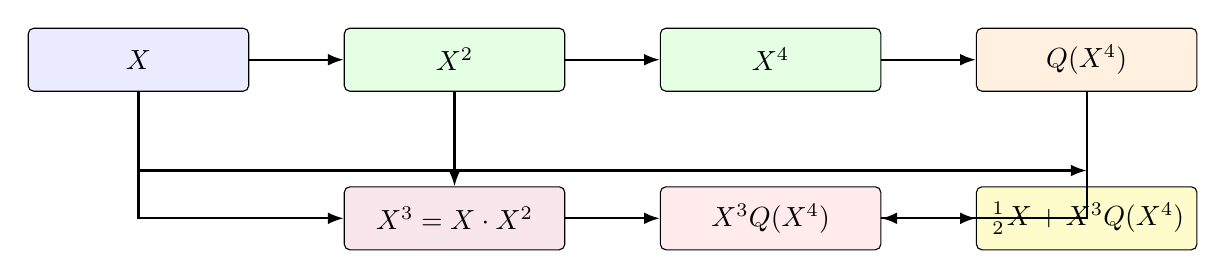
\begin{tikzpicture}[
  node distance=12mm,
  box/.style={draw, rounded corners=2pt, align=center, minimum height=8mm, minimum width=28mm},
  arr/.style={-{Latex[length=2mm]}, thick}
]
\node[box, fill=blue!8] (x) {$X$};
\node[box, fill=green!10, right=of x] (x2) {$X^2$};
\node[box, fill=green!10, right=of x2] (x4) {$X^4$};
\node[box, fill=orange!12, right=of x4] (q) {$Q(X^4)$};
\node[box, fill=purple!10, below=of x2] (x3) {$X^3=X\cdot X^2$};
\node[box, fill=red!8, right=of x3] (prod) {$X^3Q(X^4)$};
\node[box, fill=yellow!20, right=of prod] (out) {$\frac12X+X^3Q(X^4)$};
\draw[arr] (x) -- (x2);
\draw[arr] (x2) -- (x4);
\draw[arr] (x4) -- (q);
\draw[arr] (x) |- (x3);
\draw[arr] (x2) -- (x3);
\draw[arr] (x3) -- (prod);
\draw[arr] (q) |- (prod);
\draw[arr] (prod) -- (out);
\draw[arr] (x) |- ($(out.north)+(0,0.20)$);
\end{tikzpicture}
\end{center}

\section{同一参数下的实际多项式对比}

本节固定实验参数
\[
  p=65537,\quad B=17,\quad
  S_A=\{hA+\ell:\ |h|,|\ell|\le 17\},
  \quad |S_A|=1225.
\]
Ma 等人的 large-\(p\) 实验库在 \(t=-1\) 的 non-power-of-\(p\) 路径中，
默认选择
\[
  A=2\lceil B_{\rm rec}\rceil+1=35,
\]
并在 \(\mathbb F_p\) 上插值得到满足
\[
  P_{35}(35h+\ell)=\ell,\qquad |h|,|\ell|\le 17
\]
的 exact cleaner。我们的 SAT/结构搜索保留同一个 bounded-support
cleaner 问题，但把 auxiliary radix 改成
\[
  A=256,\qquad 256^2\equiv -1\pmod {65537}.
\]
由此得到另一个 exact cleaner \(P_{256}\)，满足
\[
  P_{256}(256h+\ell)=\ell,\qquad |h|,|\ell|\le 17.
\]

\begin{table}[h]
\centering
\resizebox{\linewidth}{!}{%
\begin{tabular}{lrrrll}
\toprule
来源/实现 & aux & degree & nonzero & 结构 & 正确性 \\
\midrule
HElib 原生 digit polynomial & -- & \(p\) 或 \((e-1)(p-1)+1\) & 大 & 全局 \(p\)-进制抽取 & HElib 插值/CH 公式 \\
Ma large-\(p\) 默认库 & 35 & 1223 & 612 & odd powers & support 全验证 \\
本文 SAT/结构搜索 & 256 & 1223 & 307 & \(X,X^{4j+3}\) & support 全验证 \\
本文 order-four evaluator & 256 & 1223 & 307 & \(\frac12X+X^3Q(X^4)\) & 恒等式验证 \\
\bottomrule
\end{tabular}
}
\caption{同一 \(p=65537,B=17\) bounded-support 问题下的多项式形式。}
\end{table}

这里的 ``HElib 原生'' 指 \texttt{buildDigitPolynomial} 或 Chen--Han
\texttt{compute\_magic\_poly} 路径：它解决的是全局 \(p\)-进制 digit
extraction，而不是 bounded support 上的 two-coordinate cleaner。
因此它没有 \(A=35\) 或 \(A=256\) 的 support 几何结构；在大 \(p=65537\)
下直接使用会得到 degree 至少为 \(p\) 量级的多项式。我们的 baseline
实验实际比较的是 Ma large-\(p\) 库中的 bounded-support cleaner。
对应代码路径为
\begin{center}
\scriptsize
\begin{tabular}{ll}
HElib 原生: & \texttt{baselines/HElib/src/extractDigits.cpp}\\
Ma large-\(p\) 默认库: &
\texttt{baselines/BGV-Boot-for-Large-p}\\
Ma homomorphic NTT 库: &
\texttt{baselines/bgv-bootstrapping-with-homomorphic-NTT}\\
本文实现: &
\texttt{src/HElib\_auxradix\_opt/src/extractDigits.cpp}
\end{tabular}
\end{center}

另外，Polyfunctions baseline 对应 GIKV/polyfunction 路线，目录里已有的
\texttt{poly*.txt} 主要是小 \(p\) 和小 \(e\) 的 digit extraction/retain
多项式样例，不是 \(p=65537,B=17\) 的 bounded-support cleaner。Ma 的
homomorphic NTT baseline 中缓存的 \texttt{12289\_3\_ZZX.txt} 也对应另一组参数。
因而在本实验同一参数集下，可直接比较的 Ma bounded-support cleaner 是
默认 \(A=35\) 的 \(P_{35}\)；我们的 SAT/结构搜索把同一问题的 auxiliary
radix 改为 \(A=256\)。

\paragraph{Ma 默认 cleaner 的实际形式。}
记 \(P_{35}\) 为 Ma large-\(p\) 默认路径得到的多项式。它的非零指数为
所有奇数 \(1,3,\ldots,1223\)，共 \(612\) 项。前若干项和最高若干项为
\[
\begin{aligned}
P_{35}(X)
  &= 19555X -29521X^{3} +24465X^{5} -20805X^{7}+\cdots\\
  &\quad -21432X^{1217} -16629X^{1219} -23426X^{1221} -30251X^{1223} \pmod{65537}.
\end{aligned}
\]
完整 \(612\) 项系数见
\texttt{docs/cleaner\_polynomial\_forms\_p65537\_B17.json}。

\paragraph{SAT/结构搜索得到的 cleaner。}
本文搜索得到的 \(P_{256}\) 的实际形式是
\[
  P_{256}(X)=32769X+X^3Q(X^4),
\]
其中 \(32769=2^{-1}\bmod 65537\)，且 \(Q\) 有
degree \(305\)、\(306\) 个非零项。展开到 \(X\) 的多项式时，
\[
\begin{aligned}
P_{256}(X)
  &= -32768X +21468X^{3} +17854X^{7} +13974X^{11}+\cdots\\
  &\quad -3103X^{1211} -12333X^{1215} -26247X^{1219} -4553X^{1223} \pmod{65537}.
\end{aligned}
\]
对应的 \(Q\) 的前后若干项为
\[
\begin{aligned}
Q(Y)
  &= 21468 +17854Y +13974Y^{2} -16217Y^{3}+\cdots\\
  &\quad -3103Y^{302} -12333Y^{303} -26247Y^{304} -4553Y^{305} \pmod{65537}.
\end{aligned}
\]

\paragraph{正确性。}
两个 cleaner 的正确性都不是抽样测试，而是在全部 \(1225\) 个 support
点上验证：
\[
  P_A(hA+\ell)=\ell,\qquad |h|,|\ell|\le 17.
\]
对于 \(A=256\)，还验证了 order-four 恒等式
\[
  P_{256}(256X)+256P_{256}(X)=256X
\]
在全部 support 上成立；因为两边次数都小于 \(|S_A|=1225\)，这个 support
恒等式也等价于低次数代表元中的多项式恒等式。

\paragraph{节省的 cost。}
从多项式本身看，\(P_{35}\) 到 \(P_{256}\) 把非零单项式数从 \(612\)
降到 \(307\)，减少
\[
  1-\frac{307}{612}=49.84\%.
\]
order-four evaluator 不再直接对 degree \(1223\) 的 \(P\) 做通用求值，
而是先算 \(X^2,X^3,X^4\)，再对 degree \(305\) 的 \(Q(X^4)\) 求值。
按同一 Paterson--Stockmeyer 估算，generic degree-\(1223\) 路径约
73 次 ciphertext multiplication，order-four 路径约
41 次，理论乘法数减少约
\[
  1-\frac{41}{73}
  =43.84\%.
\]
以 \texttt{/home/luck/xzy/0424project/baselines/BGV-Boot-for-Large-p}
中的 Ma large-\(p\) baseline 为正式对比对象，repeat-3 实测中，
默认 \(A=35\) 的 extract 均值为 \(160.78\)s、total 均值为
\(213.10\)s。切到 \(A=256\) sparse cleaner 后，extract 为
\(147.91\)s、total 为 \(199.40\)s；再启用 order-four evaluator 后，
extract 为 \(80.77\)s、total 为 \(131.18\)s。相对该 baseline，
sparse cleaner 的 extract/total 加速分别为 \(8.01\%\) 和
\(6.43\%\)，order-four 完整路径的 extract/total 加速分别为
\(49.76\%\) 和 \(38.44\%\)。



\section{实验数字如何对应理论}

在目标参数中：
\[
  p=65537,\qquad B=17,\qquad |S_A|=1225.
\]

\begin{table}[h]
\centering
\caption{多项式结构与真实 HElib 自举时间}
\begin{tabular}{lrrrr}
\toprule
版本 & 项数 & linear2 & extract & total\\
\midrule
Ma baseline aux $A=35$ & $612$ & $45.268850$s & $160.783267$s & $213.102573$s\\
sparse aux $A=256$ & $307$ & $44.512004$s & $147.909934$s & $199.397017$s\\
$A=256$ + order-four evaluator & $307$ & $43.623283$s & $80.770389$s & $131.180978$s\\
\bottomrule
\end{tabular}
\end{table}

可以看到有两层收益：

\begin{enumerate}
  \item \textbf{代数选 radix：} $A=256$ 让 exact cleaner 从 $612$ 项降到
  $307$ 项，但次数仍为 $1223$。这是 sparsity 优化，不是 lower-degree 优化。
  \item \textbf{结构化求值：} 利用
  $P_A(X)=\frac12X+X^3Q(X^4)$ 后，真实 extraction 从 $147.909934$s
  降到 $80.770389$s。
\end{enumerate}

相对于 \texttt{/baselines/BGV-Boot-for-Large-p} 的 Ma baseline，
完整 order-four 路径的提升为：
\[
  \text{extract speedup}=49.76\%,\qquad
  \text{total speedup}=38.44\%.
\]
相对于 sparse aux $A=256$，order-four evaluator 的增量提升为：
\[
  \text{extract speedup}=45.39\%,\qquad
  \text{total speedup}=34.21\%.
\]

\section{一句话解释}

这个优化可以用一句话概括：

\begin{center}
\fbox{
\begin{minipage}{0.86\linewidth}
我们选择 $A^2=-1$，让乘以 $A$ 在 digit support 上变成 $90^\circ$ 旋转；
cleaner 必须与这个旋转兼容，因此单项式指数被四阶 character 过滤，
只剩 $X$ 和 $X^{4j+3}$。这个结构让 exact cleaner 同时更稀疏、
并且可以写成 $X^3Q(X^4)+\frac12X$ 来更快地同态求值。
\end{minipage}}
\end{center}

\section{论文 claim 边界}

讲解时建议明确下面几点，避免过度声称：

\begin{itemize}
  \item 这不是对所有 FHE bootstrapping 的全局最优。
  \item 这不是同一固定 support 下的更低次数多项式；固定 support 的最低次数
  已由 canonical representative 决定。
  \item 正确说法是：在固定 HElib large-prime BGV thin-bootstrap pipeline
  和 bounded support cleaning 问题下，选择 order-four radix，使 exact
  cleaner 稀疏，并进一步利用该结构优化同态多项式求值。
  \item 线性变换部分的 parallel coeffToSlot 是工程补充；本 PDF 讲的主数学
  来源是 cleaner 的四阶对称性。
\end{itemize}

\section{讲解提纲}

如果要给别人讲，可以按下面 5 分钟顺序：

\begin{enumerate}
  \item 先画 support：$x=hA+\ell$，cleaner 要输出 $\ell$。
  \item 说明固定 support 下多项式代表元唯一，所以不要只追求 lower degree。
  \item 选择 $A=256$，因为 $A^2=-1$，乘以 $A$ 是 $(h,\ell)\mapsto(\ell,-h)$。
  \item 推导恒等式 $P_A(AX)+AP_A(X)=AX$。
  \item 比较系数，得到只剩 $X$ 和 $X^{4j+3}$，于是
  $P_A(X)=\frac12X+X^3Q(X^4)$，最后展示实验表格。
\end{enumerate}

\end{document}
